\chapter{Fisica dei dischi proto-planetari} \label{cap:FisDischi}
I dischi proto-planetari sono delle strutture costituite da gas e polveri che orbitano attorno a stelle giovani ($\sim\,$ Myr). Tali stelle si formano in dense nubi molecolari, che sono delle regioni di spazio ( $\sim\,10 - 100$ pc) riempite da gas e polveri (massa $\sim\,10^4 - 10^6 M_{\odot}$). 
Questi complessi possono essere osservati mediante l'utilizzo di traccianti molecolari come per esempio: CO, $^{13}$CO ed NH$_3$. I composti appena nominati possono essere utilizzati con una doppia finalità: 
\begin{list}{\textbf{-}}{\setlength{\itemsep}{0cm}}
    \item determinare la struttura della nube
    \item ricavare informazioni riguardo i movimenti del materiale
\end{list}
I traccianti molecolari hanno consentito di stabilire che le "molecular clouds" hanno momento angolare non nullo in quanto il rapporto fra energia rotazionale ed energia gravitazionale è diverso da zero \parencite{Goodman1993}.
Dato che 
\begin{equation}
\beta\,\equiv\frac{E_{rot}}{\left|E_{grav}\right|} \sim 0.02, 
\label{eq:beta}
\end{equation}
le strutture che stiamo prendendo in considerazione sono caratterizzate da lenti movimenti rotatori.
Alcune regioni di queste nubi, dette cores, sono gravitazionalmente instabili e possono collassare sotto azione della propria gravità: questo processo darà luogo alla formazione di una nuova stella (vedi Figura \ref{fig:YS0}).
Dato che il materiale possiede momento angolare non nullo, il collasso in questione non potrà avvenire radialmente.

Consideriamo un elemento di fluido facente parte di un core, che supponiamo avere asse di rotazione lungo z.
Su tale elemento agisce una forza centrifuga che bilancia la componente radiale dell'attrazione gravitazionale. L'altra componente, ossia quella verticale, agisce senza essere contrastata: questo comporta la formazione di un disco sottile attorno alla proto-stella. 
L'ultima fase della formazione stellare ($\sim$10$^6$ yr) è caratterizzata da un graduale accrescimento di materiale sul corpo centrale. 

\begin{figure}[H]
  \centering
  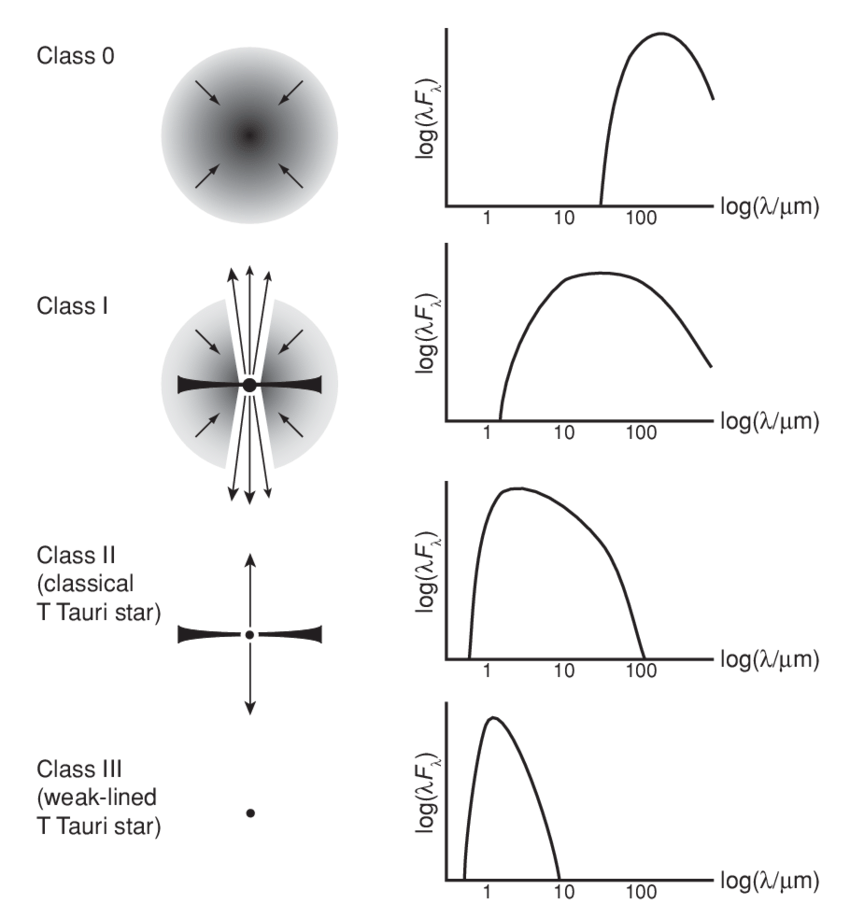
\includegraphics[width=0.9\textwidth]{Immagini/IntroTeorica/YSO.png}
  \caption{Schema riassuntivo delle fasi evolutive dei sistemi stellari giovani (YSO). Analizzando lo spettro d'emissione è possibile comprendere a che classe appartenga un generico 'young stellar object'.}
  \label{fig:YS0}
\end{figure}

Questo processo è regolato da meccanismi che determinano una ridistribuzione del momento angolare e la cui natura è ancora argomento di discussione. 
Uno dei modelli proposti identifica in fenomeni di natura viscosa ciò che sta alla base del trasporto di momento angolare \parencite{BellPringle1974}. Proposte alternative riguardano venti magnetici che sono in grado di rimuovere momento angolare, favorendo il processo d'accrescimento del materiale sulla stella \parencite{MagneticWinds}. In questa tesi lavoreremo con il modello viscoso.


\section{Modellizzazione del disco} \label{sec:mod_disc}
L'evoluzione e la struttura di un disco di accrescimento possono essere descritte utilizzando le leggi fondamentali della fluido-dinamica e della gravitazione.
Il seguente set di equazioni consente di effettuare una trattazione generale del problema che stiamo affrontando:
\begin{equation}
\partial_t \rho\,+\,\partial_j\left(\rho u^j\right)\,=\,0,
\label{eq:continuity}
\end{equation}
\begin{equation}
\partial_tu^i\,+\,\partial_j\left(u^i u^j\right)\,=\,-\frac{\partial_iP}{\rho}\,-\,\partial_i\phi\,+\,f^i,
\label{eq:Navier-Stokes}
\end{equation}
\begin{equation}
\partial_t\left(\rho e\right)\,+\,\partial_j\left(\rho e u^j\right)\,=\,-P\partial_ju^j\,+\,\rho\dot{Q},
\label{eq:energy_cons}
\end{equation}
\begin{equation}
\partial_j\partial_j\phi\,=\,-4\pi G\left[\rho\,+\,M_\ast\delta\left(r\right)\right],
\label{eq:grav_pot}
\end{equation}
dove $\rho$ è la densità del materiale costituente il disco, $u$ è la velocità, $M_\ast$ la massa della stella ed $f$ è legato ai fenomeni di natura viscosa.
La \eqref{eq:continuity} è l'equazione di continuità: essa afferma che non sono presenti nè sorgenti nè pozzi di densità, con conseguente conservazione della massa. La \eqref{eq:Navier-Stokes} è l'equazione di conservazione del momento, anche nota con il nome di equazione di Navier-Stokes. Il primo membro è analogo a quello dell'equazione di continuità, mentre il secondo descrive le varie forze che agiscono sull'elemento di fluido considerato. I termini a secondo membro rappresentano rispettivamente:
\begin{list}{\textbf{-}}{\setlength{\itemsep}{0cm}}
    \item forze di pressione
    \item forze di natura gravitazionale
    \item forze di natura viscosa
\end{list}
Per conoscere l'espressione analitica del potenziale gravitazionale $\phi$ è necessario risolvere l'equazione \eqref{eq:grav_pot}, dove figura anche la densità $\rho$ del materiale costituente il disco.
La presenza di tale termine a secondo membro è necessaria poiché il disco potrebbe essere abbastanza massivo da fornire un contributo non trascurabile a $\phi$. L'equazione \eqref{eq:energy_cons} è infine una riformulazione del primo principio della termodinamica che descrive la conservazione dell'energia e contiene un termine $\dot{Q}$ per tenere conto di ogni altra possibile sorgente di calore.
In aggiunta alle relazioni precedenti la pressione $P$, la densità $\rho$ ed $e$ sono legate fra loro dall'equazione di stato
\begin{equation}
P\,=\,\left(\gamma\,-\,1\right)\rho e,
\label{eq:eq_state}
\end{equation}
dove $\gamma$ è il coefficiente di dilatazione adiabatica.\\

La risoluzione del problema appena presentato è difficoltosa e richiederebbe elevate risorse computazionali: è possibile fare delle assunzioni che consentono di semplificare notevolmente la casistica considerata. \newpage
Il disco che tratteremo sarà:
\begin{list}{\textbf{-}}{\setlength{\itemsep}{0cm}}
    \item simmetrico per rotazioni attorno all'asse z
    \item non auto-gravitante
    \item sottile
    \item composto da gas ideale
    \item in equilibrio idrostatico lungo z
    \item verticalmente isotermo
\end{list}
Un disco proto-planetario viene detto sottile se l'estensione verticale caratteristica $h$ è molto minore della dimensione radiale cilindrica $r$. 
Per i dischi circum-stellari si ha solitamente che $h/r\,\simeq\,0.1$:  l'approssimazione che vogliamo introdurre è verificata in natura.
La condizione di disco sottile ci consente di semplificare notevolmente il problema originale: possiamo infatti integrare lungo la direzione verticale le equazioni di partenza passando da un sistema tridimensionale ad uno bidimensionale. \'E possibile mostrare che lavorare con $h/r\,\ll\,1$ equivale a richiedere che la velocità del suono $c_s$ sia molto minore della velocità di rotazione $v_{\theta}$ del materiale. Il disco che stiamo studiando è quindi dinamicamente freddo, ossia è caratterizzato da una dinamica super-sonica.

Vogliamo inoltre limitarci allo studio di dischi non auto-gravitanti: la densità $\rho$ non comparirà più a secondo membro dell'equazione di Poisson per la determinazione del potenziale gravitazionale $\phi$. La \eqref{eq:grav_pot} assumerà quindi la forma
\begin{equation}
\partial_j\partial_j\phi\,=\,-4\pi GM_\ast\delta\left(r\right),
\label{eq:grav_pot1}
\end{equation}
con soluzione
\begin{equation}
\phi(r,\,z)\,=\,-G\frac{M_\ast}{\sqrt{r^2\,+\,z^2}}.
\label{eq:pot_form1}
\end{equation}
Sfruttando che $h/r\,\ll\,1$ è possibile trascurare la presenza di $z^2$ ad argomento della radice, ottenendo un potenziale gravitazionale con dipendenza solo sulla coordinata radiale cilindrica.

\subsection{Viscosità} \label{subsec: viscosity}

Prima di discutere in dettaglio le caratteristiche dei dischi è necessario investigare la natura dei fenomeni viscosi.
La viscosità molecolare in questi sistemi è trascurabile, poiché i tempi d'evoluzione se essa fosse l'unica forma di viscosità presente sarebbero dell'ordine di $10^{13}$ anni, ossia milioni di volte superiori a quanto osservato.
Le turbolenze presenti all'interno del disco possono fornire delle viscosità efficaci nettamente più intense di quella molecolare \parencite{ShakuraAlfaPer}.
Per turbolenze isotrope, la massima scala su cui esse si possono sviluppare è dello stesso ordine di grandezza della dimensione verticale del disco $h$. 
La massima velocità dei movimenti turbolenti sarà la velocità del suono, perché avere $u\,>\,c_s$ porterebbe a shock associati a rapida dissipazione dell'energia in calore. 
Queste considerazioni motivano la parametrizzazione
\begin{equation}
\nu\,=\,\alpha c_s h,
\label{eq:alfa_par}
\end{equation}
dove $\alpha$ è un parametro adimensionale che indica quanto efficiente sia il trasporto del momento angolare.
Per i dischi i valori di $\alpha$ universalmente accettati variano da $10^{-4}$ fino a $10^{-2}$: il range appena indicato è quello che procederemo ad analizzare in questa tesi.

\subsection{Struttura verticale} \label{subsec:str_vert_disc}

Il profilo di densità verticale si ricava a partire dall'assunzione di equilibrio idrostatico lungo la direzione z. Consideriamo un elemento di fluido posto a distanza radiale $r$ e ad altezza $z$ rispetto al piano equatoriale. 
Tale porzione del disco è in equilibrio lungo l'asse z se la forza di pressione e quella di gravità si bilanciano
\begin{equation}
\frac{dP}{dz}\,=\,-\rho g_z.
\label{eq:idrostatic_eq}
\end{equation}
La componente verticale dell'accelerazione di gravità si ottiene con delle semplici considerazioni geometriche (vedi Figura \ref{fig:costr_geom}):
\begin{equation}
g_z\,=\,\frac{GM_\ast}{r^2\,+\,z^2}\sin{\left(\theta\right)}\,=\,\frac{GM_\ast}{d^3}z
\label{eq:vertical_g}
\end{equation}
\begin{figure}[H]
    \centering
    \includegraphics[height=5cm, width=12cm]{Immagini/IntroTeorica/GravitàVert.png}
    \caption{Costruzione geometrica per la determinazione del profilo di densità verticale}
    \label{fig:costr_geom}
\end{figure}
Nel limite in cui $z\ll r$ è possibile approssimare l'espressione precedente sfruttando che $r\sim d$. Sostituendo la coordinata radiale al posto della distanza fra l'elemento di fluido considerato e la stella, otteniamo una relazione in cui è possibile riconoscere la velocità angolare kepleriana $\Omega$.
\begin{equation}
g_z\,\simeq\,\frac{GM_\ast}{r^3}z\,=\,\Omega^2 z
\label{eq:vertical_g_1}
\end{equation}
Supponiamo ora per semplicità che il disco sia verticalmente isotermo: l'equazione di stato che lega la pressione alla densità del gas è di conseguenza
\begin{equation}
P\,=\,\rho c_s^2,
\label{eq:isothermal}
\end{equation}
dove $c_s$ indica la velocità del suono. Sostituendo le relazioni per la pressione e la componente verticale dell'accelerazione gravitazionale nell'equazione per l'equilibrio idrostatico (\ref{eq:idrostatic_eq}) è possibile ricavare l'equazione differenziale
\begin{equation}
\frac{d\rho}{dz}\,=\,-\rho \left(\frac{\Omega}{c_s}\right)^2 z.
\label{eq:eq_diff_rho}
\end{equation}
La soluzione  di \eqref{eq:eq_diff_rho} è una gaussiana:
\begin{equation}
\rho (z)\,=\,\rho_0 \exp\left(-\frac{z^2}{2h^2}\right)
\label{eq:dens_prof}
\end{equation}
dove $h\,=\,c_s/\Omega$ indica la scala d'altezza verticale. Può risultare utile dividere $h$ per la coordinata radiale: il rapporto che si ottiene è detto aspect-ratio ed esplicita come vari la scala d'altezza in funzione della distanza dalla stella.
\begin{equation}
\frac{h}{r}\,=\,\frac{c_s}{v_\theta}
\label{eq:aspect_ratio}
\end{equation}
L'aspect-ratio consente di dividere i dischi in due categorie:
\begin{list}{\textbf{-}}{\setlength{\itemsep}{0cm}}
    \item dinamicamente freddi, caratterizzati da $h/r\,<\,1$
    \item dinamicamente caldi, dove invece $h/r\,\gtrsim\,1$
\end{list}
I primi sono caratterizzati da una dinamica super-sonica, con onde sonore che si propagano a velocità inferiori di quelle di movimento del gas. La dinamica nei dischi del secondo tipo è invece di natura sub-sonica.

La discussione precedente ha consentito di esplicitare un legame fra lo spessore del disco e la temperatura $T$ del materiale: si ha infatti che
\begin{equation}
c_s \propto \sqrt{T}.
\label{eq:vsuono_T}
\end{equation}
L'origine fisica di questa dipendenza è dovuta al fatto che il gradiente di pressione contrasta l'effetto della gravità consentendo un'estensione verticale più grande: più caldo è il disco, maggiore è l'effetto che si ottiene. La determinazione della forma del disco è possibile solamente se è noto il legame fra $T$ ed $r$.

\subsection{Profilo di temperatura}

Per ottenere il profilo di densità verticale abbiamo lavorato assumendo il disco verticalmente isotermo: $T$ può ancora essere funzione della coordinata radiale.
Le fonti di riscaldamento del disco sono principalmente due:
\begin{list}{\textbf{-}}{\setlength{\itemsep}{0cm}}
    \item luce stellare intercettata dal disco (solitamente dalle polveri che ne fanno parte)
    \item dissipazione di energia potenziale gravitazionale, poiché si ha accrescimento di materiale sulla stella
\end{list}
I dischi per i quali il processo principale è il primo sono detti dischi passivi. Se a dominare è invece il secondo fenomeno, il disco è detto attivo.
Questa distinzione è una chiara semplificazione di quanto accada in realtà. La sorgente principale di calore per un disco è una funzione sia del tempo che della posizione: ci aspettiamo che nelle fasi iniziali dell'evoluzione e a piccoli raggi dominino meccanismi di riscaldamento interno, mentre a tempi successivi e in punti più esterni sia fonte principale la luce della stella. Il meccanismo che determina il raffreddamento del disco è l'emissione di corpo nero da parte della polvere.

I tempi caratteristici per il raggiungimento dell'equilibrio termico sono molto più brevi di quelli caratterizzanti l'evoluzione del disco oppure della stella. Il profilo di temperatura è allora determinato dal bilanciamento fra assorbimento ed emissione di calore.\\

\textbf{Riscaldamento radiativo}\\

Il profilo di temperatura di un disco passivo è strettamente legato all'estensione spaziale del disco stesso: al variare della forma, cambia anche la quantità di radiazione stellare che può essere intercettata. Limitiamoci allo studio di un sistema costituito da un disco piatto e sottile che assorba tutta la radiazione che lo colpisce e che localmente emetta come se fosse un corpo nero. Lavoriamo con un sistema di riferimento sferico e con una stella modellizzata come una sfera di raggio $R_{\ast}$ con temperatura efficace $T_{\ast}$ costante nel tempo. Per un tale corpo celeste la brillanza superficiale $I_\ast$ risulta
\begin{equation}
I_\ast\,=\,\sigma T_\ast^4, 
\label{eq:lum_star}
\end{equation}
dove $\sigma$ è la costate di Stefan-Boltzmann.

Per poter determinare l'andamento di $T_{disco}\left(r\right)$ dobbiamo ora valutare quale sia il flusso di radiazione incidente. 
Lavorando con coordinate polari sferiche, come mostrato in Figura \ref{fig:temp_pass}, il flusso passante per un elemento di superficie a distanza $r$ dalla stella è pari a
\begin{equation}
F\,=\,\int I_\ast \sin{\theta} \cos{\phi} d\Omega.
\label{eq:in_flux}
\end{equation}

\begin{figure}[H]
    \centering
    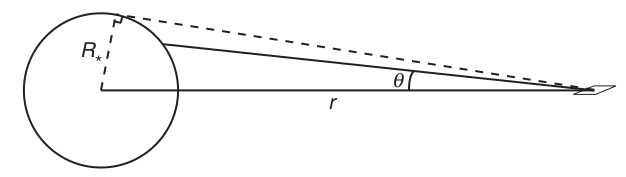
\includegraphics[height=4cm, width=10cm]{Immagini/IntroTeorica/Temp_Pass.png}
    \caption{Costruzione geometrica utilizzata per calcolare il flusso incidente su un disco piatto e sottile \parencite{Dispense}}
    \label{fig:temp_pass}
\end{figure}
Dato che il problema che stiamo considerando è simmetrico rispetto al piano equatoriale, consideriamo solamente la radiazione emessa dalla metà superiore della stella. I limiti di integrazione sono quindi:
\begin{equation}
-\pi/2\,<\,\phi\,\leq\pi/2,
\label{eq:flux_lim_phi}
\end{equation}
\begin{equation}
0\,<\,\theta\,<\arcsin{\left(\frac{R_\ast}{r}\right)}
\label{eq:flux_lim_phi}
\end{equation}
Svolgendo l'integrale \eqref{eq:in_flux} si ottiene che
\begin{equation}
F\,=\,I_\ast\left[\arcsin{\left(\frac{R_\ast}{r}\right)}\,-\,\frac{R_\ast}{r}\sqrt{1\,-\,\left(\frac{R_\ast}{r}\right)^2}\right].
\label{eq:ex_flux}
\end{equation}
Dato che il disco si trova all'equilibrio termico, uguagliamo $F$ all'emissione di corpo nero $\sigma T_{disco}^4$ ottenendo che
\begin{equation}
T_{disco}\left(r\right)\,=\, \left\{\frac{I_\ast}{\sigma}\left[\arcsin{\left(\frac{R_\ast}{r}\right)}\,-\,\left(\frac{R_\ast}{r}\right)\sqrt{1\,-\,\left(\frac{R_\ast}{r}\right)^2}\right]\right\}^{1/4}.
\label{eq:radial_prof}
\end{equation}
Notiamo che per $R_\ast/r\,\ll\,1$ la relazione fra temperatura del disco e coordinata radiale è del tipo $T_{disco}\propto r^{-3/4}$.\\

\textbf{Riscaldamento viscoso}\\

Per determinare $T_{disco}\left(r\right)$ nel caso di un disco attivo dobbiamo studiare i fenomeni di natura viscosa che determinano la dissipazione di energia potenziale gravitazionale. Consideriamo un anellino di spessore $\Delta r$. Il momento torcente netto su tale regione del disco sprigiona una potenza pari a
\begin{equation}
\Omega \frac{\partial G}{\partial r} \Delta r \equiv \left[\frac{\partial}{\partial r}\left(G\Omega\right)\,-\,G\frac{d\Omega}{dr}\right] \Delta r.
\label{eq:work_torque}
\end{equation}
Supponiamo ora di considerare l'intero disco, ossia di integrare rispetto ad $r$ la \eqref{eq:work_torque}. Notiamo che il primo termine del secondo membro sarebbe determinato solamente dai valori assunti agli estremi di integrazione: identifichiamo questo temine con il trasporto di energia associato ai momenti torcenti viscosi.
Il secondo termine è di natura dissipativa e rappresenta il tasso di trasmissione di energia al gas. Assumiamo che questa venga convertita in calore e irradiata,  così che il tasso di dissipazione per unità di area del disco risulti essere
\begin{equation}
D\left(r\right)\,=\,\frac{G}{4\pi r} \frac{d\Omega}{dr}\,=\,\frac{9}{8}\nu\Sigma\Omega^2, 
\label{eq:diss_visc}
\end{equation}
dove abbiamo assunto un profilo di velocità Kepleriano. Per un corpo nero sappiamo che $D\left(r\right)\,=\,\sigma T_{disco}^4$. Imponendo l'equilibrio otteniamo
\begin{equation}
T^4_{disco}\,=\,\frac{3GM_\ast\dot{M}}{8\pi\sigma r^3}\left(1\,-\,\sqrt{\frac{R_\ast}{r}}\right),
\label{eq:ptemp_act}
\end{equation}
dove $\dot{M}$ indica il tasso di accrescimento sulla stella. Notiamo che il profilo di temperatura che abbiamo ottenuto non ha alcuna dipendenza dalla viscosità del disco, ma è legato a $\dot{M}$. Come nel caso precedentemente analizzato, per $R_\ast/r \ll 1$ si ha che: $T_{disco} \propto r^{-3/4}$\\

\'E necessario sottolineare che i risultati esposti in precedenza non sono auto-consistenti. Per semplificare la casistica trattata abbiamo lavorato con dei dischi piatti ottenendo che $T_{disco} \propto r^{-3/4}$: questa dipendenza fa sì che la velocità del suono $c_s \propto r^{-3/8}$. 
Utilizzando la \eqref{eq:aspect_ratio} notiamo che $h/r \propto r^{1/8}$: il disco tenderà ad espandersi maggiormente nelle regioni esterne andando ad intercettare più luce. Le zone a grandi raggi presenteranno quindi una fonte di calore maggiore: il profilo di temperatura non potrà avere una caduta così repentina. 
\'E stato verificato che in un disco passivo 'flared' la temperatura a grandi distanze ha un andamento del tipo $T\left(r\right)\propto r^{-1/2}$ \parencite{KenyonHartmann1987}

\section{Evoluzione del disco}

I dischi non sono delle strutture statiche, ma evolvono lentamente nel tempo. Per un disco geometricamente sottile la velocità angolare è essenzialmente quella di un orbita Kepleriana. 
Questo implica che il momento angolare specifico $l\,=\,\sqrt{GM_\ast r}$ è una funzione crescente del raggio: per far sì che il materiale possa fluire verso l'interno deve necessariamente perdere momento angolare. Secondo il modello viscoso, l'evoluzione di $\Sigma\left(r,\,t\right)$ può essere determinata \parencite{Pringle1981} componendo l'equazione di continuità
\begin{equation}
r\frac{\partial\Sigma}{\partial t}\,+\,\frac{\partial}{\partial r}\left(r\Sigma v_r\right)
\label{eq:cont_eq_cil}
\end{equation}
con l'equazione per la conservazione del momento angolare
\begin{equation}
r\frac{\partial}{\partial t}\left(r^2\Omega\Sigma\right)\,+\,\frac{\partial}{\partial r}\left(r^3\Omega\Sigma v_r\right)\,=\,\frac{1}{2\pi}\frac{\partial G}{\partial r}.
\label{eq:cons_moma}
\end{equation}
La \eqref{eq:cons_moma} deriva direttamente dalla componente azimutale dell'equazione di Navier-Stokes.
Per un fluido viscoso il momento torcente $G$ applicato su un anellino è dato dal prodotto fra la circonferenza, la forza viscosa per unità di lunghezza ed il braccio della forza. Possiamo allora esplicitare $G$ come
\begin{equation}
G\,=\,2\pi r \cdot \nu\Sigma r \frac{d\Omega}{dr} \cdot r,
\label{eq:torque_vis}
\end{equation}
dove $\nu$ è la viscosità cinematica. Procediamo ora combinando la \eqref{eq:cont_eq_cil} con la \eqref{eq:cons_moma} con l'obiettivo di eliminare la velocità radiale $v_r$. Concentrandosi su un potenziale di tipo Kepleriano, ossia tale per cui $\Omega\,\propto\,r^{-3/2}$, è possibile ottenere una relazione che descriva l'evoluzione della densità superficiale di un disco geometricamente sottile:
\begin{equation}
\frac{\partial \Sigma}{\partial t}\,=\,\frac{3}{r}\frac{\partial}{\partial r}\left[r^{1/2} \frac{\partial}{\partial r}\left(\nu\Sigma r^{1/2}\right)\right]
\label{eq:master_eq}
\end{equation}
La \eqref{eq:master_eq} è un'equazione di diffusione. Una volta effettuato il seguente cambio di variabili
\begin{equation}
X\,\equiv 2r^{1/2}
\label{eq:var_x_ch}
\end{equation}
\begin{equation}
f \equiv \frac{3}{2} \Sigma X
\label{eq:var_y_ch}
\end{equation}
si presenta infatti nella tipica forma
\begin{equation}
\frac{\partial f}{\partial t}\,=\,D\frac{\partial^2 f}{\partial X^2}
\label{eq:diff_ev}
\end{equation}
con coefficiente di diffusione
\begin{equation}
D\,=\,\frac{12\nu}{X^2}.
\label{eq:diff_coeff}
\end{equation}\\
In generale $\nu$ sarà una funzione delle condizioni locali del disco.
Soluzioni analitiche sono possibili se $\nu$ presenta una dipendenza polinomiale nei confronti della coordinata radiale \parencite{BellPringle1974}.
Nel caso in cui la viscosità cinematica dipenda dalla densità superficiale $\Sigma$ allora l'equazione di evoluzione diventa non lineare e più problematica da risolvere.

\subsection{Caso particolare: spreading ring}\label{sec:spreading-ring}

Lavoriamo con $\nu$ costante. Supponiamo che la condizione iniziale consista in un anello infinitesimamente sottile di massa $m$. La densità superficiale è allora descritta da una $\delta$ centrata in una certa posizione radiale $R_0$:
\begin{equation}
\Sigma\left(r,\,t\,=\,0\right)\,=\,\frac{m}{2\pi R_0}\delta\left(r\,-\,R_0\right).
\label{eq:condin_sp_ring}
\end{equation}
\'E possibile mostrare \parencite{BellPringle1974} che la soluzione dell'equazione di evoluzione diffusiva è
\begin{equation}
\Sigma\left(x,\,\tau\right)\,=\,\frac{m}{\pi r_0^2} \frac{1}{\tau} x^{-1/4}\exp{\left(-\frac{1\,+\,x^2}{\tau}\right)}I_{1/4}\left(\frac{2x}{\tau}\right),
\label{eq:sol_sp_ring}
\end{equation}
dove $x \equiv r/R_0$, $\tau \equiv 12\nu R_0^{-2}t$ ed $I_{1/4}$ è una funzione di Bessel modificata del primo tipo. L'evoluzione del profilo di densità radiale è riportato in Figura \ref{fig:ev_sp_disc}. 
Sotto l'azione di forze di natura viscosa il disco si espande sia verso l'interno che verso l'esterno. L'allargamento verso l'esterno è necessario per la conservazione del momento angolare.

\begin{figure}[H]
    \centering
    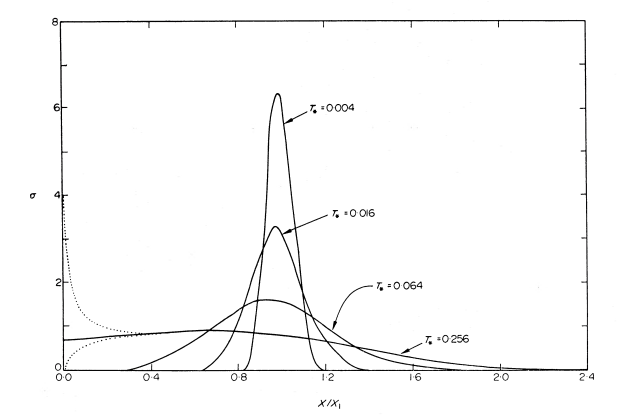
\includegraphics[height=9cm, width=12cm]{Immagini/IntroTeorica/EvoluzioneAnello.png}
    \caption{Soluzione dell'equazione di evoluzione del disco con $\nu\,=\,const$. Si nota l'allargamento dell'anello inizialmente orbitante al raggio $R\,=\,R_0$. Sono riportati profili di densità a quattro tempi differenti:$\tau\,=\,0.004$, $\tau\,=\,0.016$, $\tau\,=\,0.064$, $\tau\,=\,0.256$. \parencite{BellPringle1974}}
    \label{fig:ev_sp_disc}
\end{figure}

Per $t\,\rightarrow\,\infty$ si ha che:
\begin{list}{\textbf{-}}{\setlength{\itemsep}{0cm}}
    \item la massa si sposta verso $r\,=\,0$, con conseguente accrescimento del materiale sul corpo centrale.
    \item il momento angolare, trasportato da una frazione di massa trascurabile, viene portato verso $r\,=\,\infty$. Durante l'evoluzione viscosa del disco $L$ è conservato.
\end{list}

\subsection{Caso particolare: self similar solution}

Consideriamo un disco con viscosità $\nu \propto r^{\gamma}$. Supponiamo che la densità di materiale al tempo $t\,=\,0$ sia quella dello stato stazionario fino ad $r/r_1\,=\,\tilde{r}\,=\,1$ e che per posizioni radiali oltre $r_1$ presenti un cut-off di tipo esponenziale:
\begin{equation}
\Sigma\left(t\,=\,0\right)\,=\,\frac{C}{3\pi \nu(r_1)\tilde{r}^{\gamma}}\exp{\left(-\Tilde{r}^{2\,-\,\gamma}\right)}.
\label{eq:condin_sss}
\end{equation}
La soluzione dell'equazione di evoluzione del disco \eqref{eq:master_eq} è graficata in Figura \ref{fig:Self_Similar}
\begin{figure}[H]
    \centering
    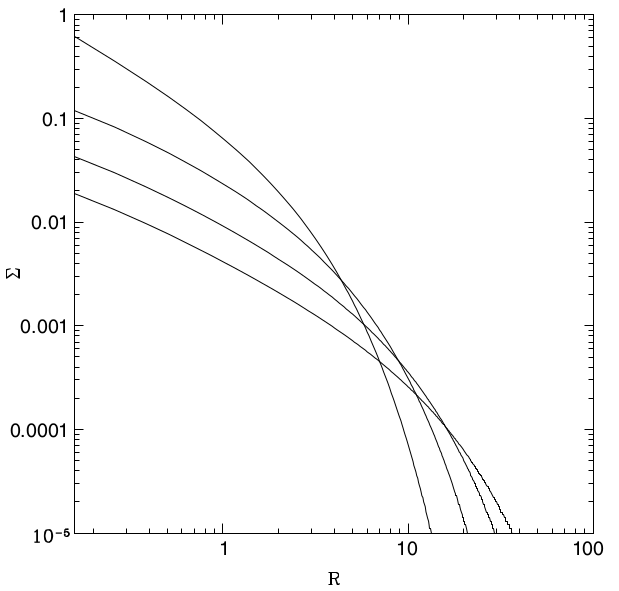
\includegraphics[height=8cm, width=10.5cm]{Immagini/IntroTeorica/SelfSimilarSolution.png}
    \caption{Soluzione dell'equazione di evoluzione del disco con $\nu\,=\,r^\gamma$. Si nota l'aumento della scala caratteristica del disco al passare del tempo \parencite{Lodato2008}.}
    \label{fig:Self_Similar}
\end{figure}
ed ha espressione analitica
\begin{equation}
\Sigma\left(\Tilde{r},\,T\right)\,=\,\frac{C}{3\pi\nu(r_1)\tilde{r}^\gamma}T^{-(5/2-\gamma)/(2-\gamma)}\exp{\left(-\frac{\Tilde{r}^{2-\gamma}}{T}\right)}, 
\label{eq:sol_sss}
\end{equation}
dove:
\begin{equation}
T \equiv \frac{t}{t_s}\,+\,1
\label{eq:T_sss}
\end{equation}
\begin{equation}
t_s \equiv \frac{1}{3\left(2\,-\,\gamma\right)^2} \frac{r_1^2}{\nu(r_1)}
\label{eq:ts_sss}
\end{equation}
\'E possibile osservare come la massa del disco diminuisca a causa dell'accrescimento di materiale sulla stella, mentre l'estensione spaziale dello stesso aumenta in modo tale da conservare il momento angolare.